\section{Aufgabe 16}
\setcounter{section}{16}

Es sei $f : \mathbb{R} \rightarrow \mathbb{R}$, $f(x) = x^3 + ax$, $a \in \mathbb{R}$.

\begin{enumerate}[(a)]
    \item Skizzieren Sie jeweils den Graph von $f$ f"ur $a = 1$ und $a = -2$.
        \begin{figure}[h]
            \centering
            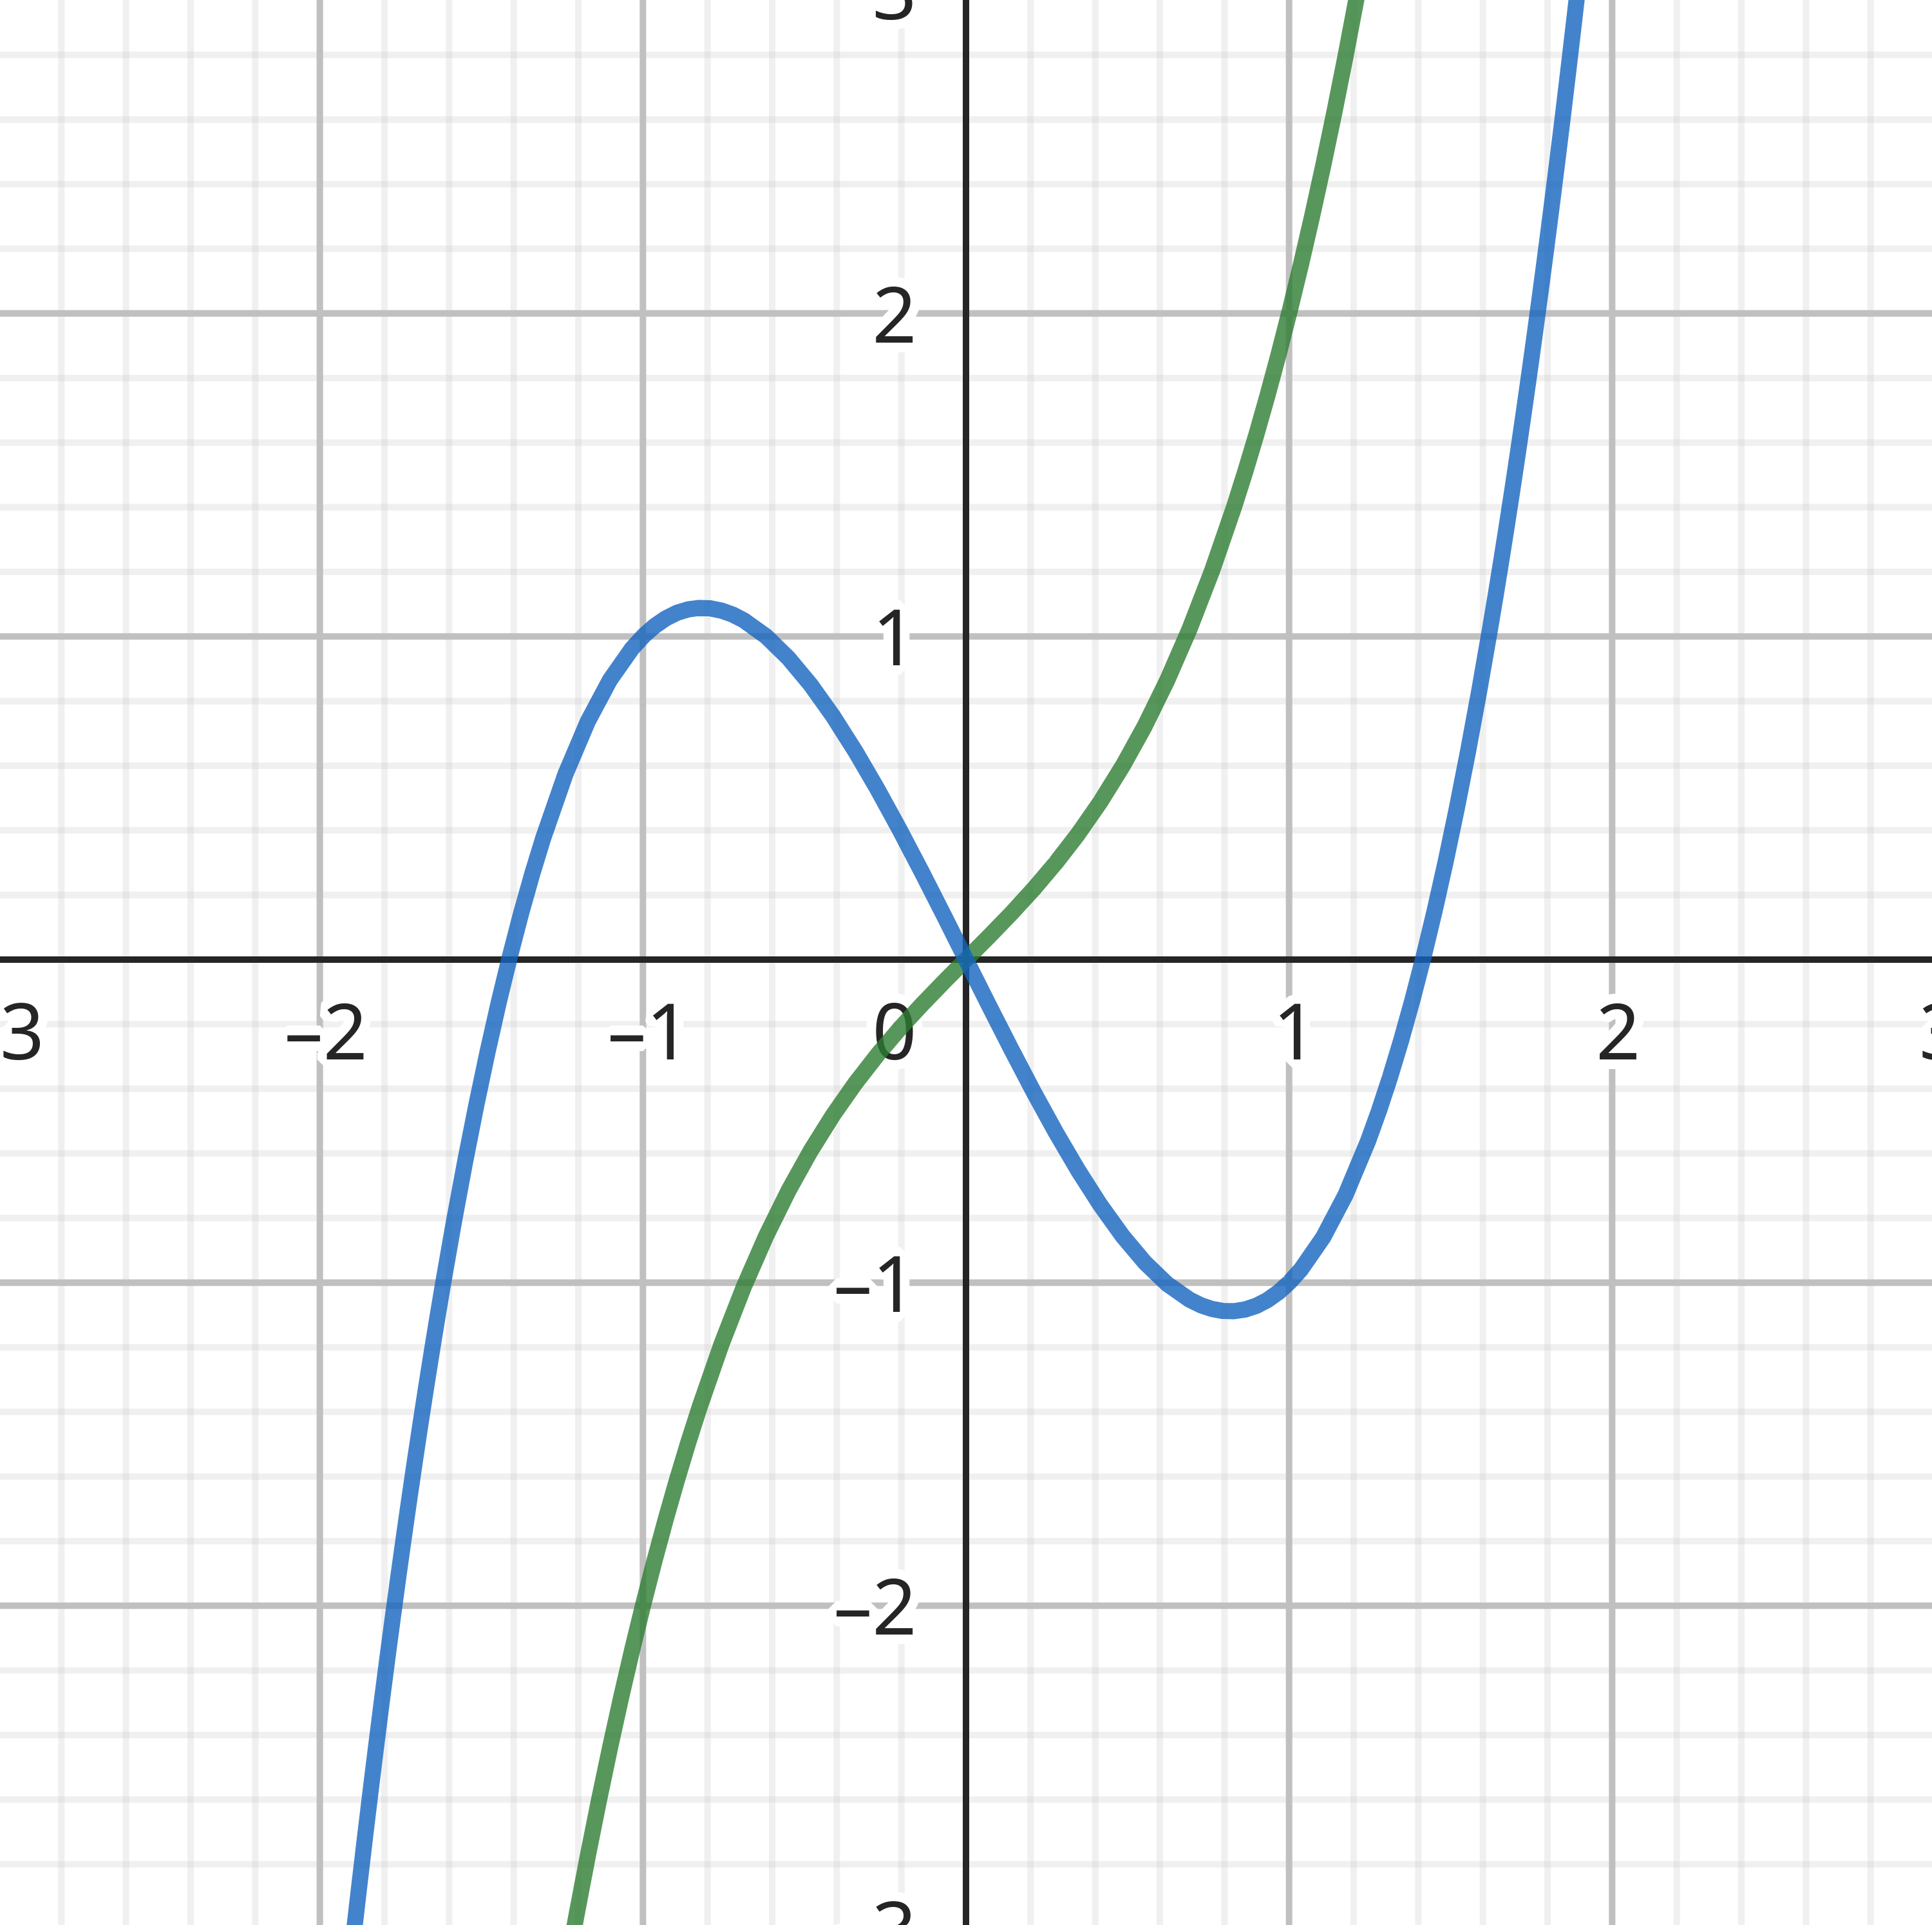
\includegraphics[width=0.40\textwidth]{./assets/abbildung-16-01.png}
            \caption{}
        \end{figure}

    \item Zeigen Sie, dass f"ur $a < 0$ die Abbildung $f$ nicht injektiv ist.

        Eine Funktion $f$ ist nicht injektiv, wenn
        \begin{equation*}
            \exists x_1, x_2 \in X, x_1 \neq x_2 \implies f(x_1) = f(x_2)
        \end{equation*}
        Setzen wir $f(x_1) = f(x_2)$, so erhalten wir:
        \begin{equation*}
            \begin{array}{rcl}
                x_1^3 + ax_1 &=& x_2^3 + ax_2 \\[5pt]
                x_1^3 - x_2^3 &=& -a(x_1 - x_2)  \\[10pt]
                \dfrac{x_1^3 - x_2^3}{x_1 - x_2} &=& -a \\[15pt]
                \dfrac{x_1^3 - x_2^3}{x_1 - x_2} &>& 0 \\[15pt]
                -a &>& 0 \\[5pt]
                 a &<& 0
            \end{array}
        \end{equation*}
\end{enumerate}
